% Chapter 3

\chapter{Probing the origins of the satellite galaxy distribution in central haloes.} 
\label{Chapter:GalDist}
\lhead{Chapter 3. \emph{Satellite Distributions}} % Write in your own chapter title to set the page header
\begin{center}
    \textit{With more purpose than the course your life was on \newline
    But if you haven't seen the places you have come from\newline
    Then you haven't seen how far you have come\newline
    In the bigger picture, there's a star sixteen times fainter\newline
    In the bigger picture, there's a course seventeen times straighter\newline
    In the bigger picture, there's a dream eighteen times greater\newline
    And it'll steer you like no other, in the bigger picture...\newline}
Stornoway - `The Bigger Picture'
\end{center}


\section{Background}
%What do we know about the distributions of galaxies
In the \LCDM model of the universe growth of haloes is hierarchical. Haloes over time acquire a substructure of accreted haloes. Given each halo is thought to contain a galaxy at its centre the halo substructure implies that galaxies should be similarly arranged. The potential application of this is that satellite galaxies situated can, therefore, be used as tracers of dark matter and used to constrain the cosmological parameters within a given \LCDM cosmology. However, to be a reliable method of predicting the distribution of dark matter and a good test of \LCDM cosmology a robust model of the connection between dark matter assembly and satellite galaxies is required.

In this chapter, we explore the ability of \steel to reproduce satellite distributions over multiple epochs. By exploiting the transparent nature of semi-empirical modelling and the flexibility of \steel we probe the impact on satellite galaxy distributions of changing: the dynamical friction timescale, stripping of satellite stellar mass, and star formation rate. In turn, probing the strength of these effects which are crucial to understanding the nature of satellites and their mergers with central galaxies.  

\section{Halo Structure and Dynamical Friction}

To constrain the evolution of the subhalo/galaxy population we need to isolate which subhalo mass bins from the unevolved subhalo accretion history have yet to finish their dynamical friction timescale and thus have survived to following epochs. The sum of all the surviving subhaloes (at each epoch) then yields the unevolved surviving subhalo mass function (USSHMF). 

\subsection{Sub-halo Merging Timescale}
\label{sec:Timescale}
 A key parameter used to calculate the unevolved surviving SHMF is the ``observability timescale'' (or survival time) of each  subhalo mass bin $[M_{h,sat}(z),$ $M_{h,sat}(z) + dM_{h,cent}(z)]$ associated to a parent halo mass bin $[M_{h,cent}(z),$ $M_{h,cent}(z) + dM_{h,cent}(z)]$. This timescale is equivalent to the merger timescale $\tau_{merge}$ of a subhalo of mass $M_{h,sat}$ in a parent halo mass $M_{h,cent}$, which is extracted from numerical simulations and represents the (average) time a subhalo ``survives'' orbiting within the parent halo. To calculate $\tau_{merge}$ we use the routines in Equation \ref{eqn:Tmerge} derived from N-body simulations \citep{Boylan-Kolchin2008},

\begin{equation}
\label{eqn:Tmerge}
\tau_{merge} =
(f_{t_{dyn}}\tau_{dyn}) \frac{A(M_{h, cent}/M_{h,sat})^B}{\ln(1+M_{h, cent}/M_{h, sat})} \exp \Big(C\frac{J}{J_c(E)}\Big) \Big( \frac{r_c(E)}{r_{vir}} \Big)^D,
\end{equation}

where A=0.9, B=1.0, C=0.6, D=0.1 \citep{McCavana2012TheMergers}. The factor $\tau_{dyn}$ is given by \citep{Jiang2016StatisticsFunctions},

\begin{equation}
\label{eqn:tdyn}
%t_{dyn} = N \cdot 0.1 \cdot {H(z)}^{-1} 
\tau_{dyn} = 1.628 h^{-1} \mathrm{Gyr} \Big(\frac{\Delta_{vir}(z)}{178}\Big)^{-\frac{1}{2}} \Big(\frac{H(z)}{H_0}\Big)^{-1} \, .
\end{equation}

Our method of considering average halo mass and accretion histories does not permit tracking single orbits and associated orbital energies. We assume instead an average orbit circularity of 0.5 \citep{Khochfar2006OrbitalHalos}, thus reducing the dependence on the angular momentum and radial components, $\frac{J}{J_c(E)}$ and $\frac{r_c(E)}{r_{vir}}$, to a constant. In other words, this approximation is consistent with the approach of taking the average expected orbits of subhaloes at fixed parent halo mass.
The key parameter of our analysis is the factor $f_{t_{dyn}}$ included in Equation \ref{eqn:Tmerge}.
The fudge factor $f_{t_{dyn}}$ takes into account the systematic uncertainties induced by numerical resolution effects in N-body simulations which are unable to resolve the full merging timescales of subhaloes and/or the satellite galaxies they host \citep{vandenBosch2018DisruptionFiction}. The parameter $f_{t_{dyn}}$ increases or decreases the dynamical times of  ``merging'' satellites enabling an exploration of the effect of dynamical time on the final number density distributions of satellite galaxies at any given epoch.

\subsection{Surviving Subhalo Population}
At each redshift we use the unevolved subhalo accretion history and the observability timescale $\tau_{merge}$ to calculate the total `observable' subhalo population associated with any given parent halo mass bin $[M_{h,cent}(z),$ $M_{h,cent}(z) + dM_{h,cent}(z)]$, i.e. the unevolved surviving SHMF (shown by the dashed lines in Figure \ref{fig:SHMF_clus}). To compute the implied total number densities of unmerged subhaloes with mass $[M_{h,sat}(z),$ $M_{h,sat}(z) + dM_{h,sat}(z)]$ at any redshift of interest we convolve the unevolved surviving SHMF with the HMF,

\begin{equation}
\label{eqn:GSHMF}
N(M_{h, sat}, z) =
\int USSHMF\Bigg(\frac{M_{h, sat}}{M_{h, cent}}\Bigg)HMF(M_{h, cent}, z)dM_{h, cent}.
\end{equation}

Figure \ref{fig:SHMF} shows the total observable subhalo population for different  $f_{t_{dyn}}$ similar to the SHMF in Figure \ref{fig:SHMF_clus}. Furthermore, via appropriate abundance matching algorithms, we can assign corresponding satellite galaxies to the unevolved subhalo accretion history and obtain the distribution of satellites in a given parent halo mass bin $[M_{h,cent}(z),$ $M_{h,cent}(z) + dM_{h,cent}(z)]$ by assuming the satellites follow the same merging timescales as their host subhaloes.

\begin{figure}
    \centering
    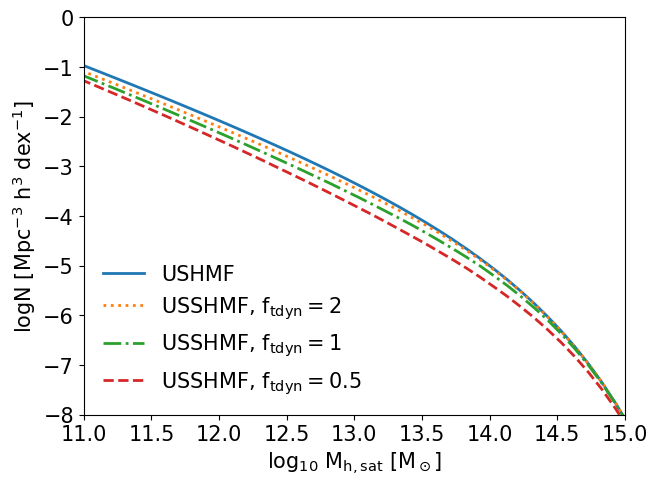
\includegraphics[width = \linewidth]{Figures/Chapter3/SHMF.png}
    \caption{Example of the `total' unevolved SHMF (solid line) and three `total' unevolved surviving SHMF (dotted lines) corresponding to three different $f_{t_{dyn}}$ factors.}
    \label{fig:SHMF}
\end{figure}

\section{Observed Satellite Distributions}
\label{sec:ObsSatDist}
As shown in Equations \ref{eqn:Tmerge} and \ref{eqn:tdyn} the dynamical friction/observability timescale is dependent on the ratio of halo to subhalo mass. In Figure \ref{fig:Tdyn_M} in the left-hand panel the merging timescales for subhaloes falling into three different central masses at redshift $z=3$ are shown. In each case, smaller subhaloes, with lower mass ratios, have longer merging times. For subhaloes that are significantly under an order of magnitude of the mass of the central halo, the merging timescales are longer then the age of the Universe and such objects would still be present in halo structures today. Through the association of galaxies to subhaloes, via the SMHM relationship at infall, we can repeat the exercise with satellite galaxies. It is similarly found that small galaxies in massive haloes are the only galaxies accreted at redshift $z = 1.5$ that are still orbiting local galaxies.

\begin{figure}[h]
    \centering
    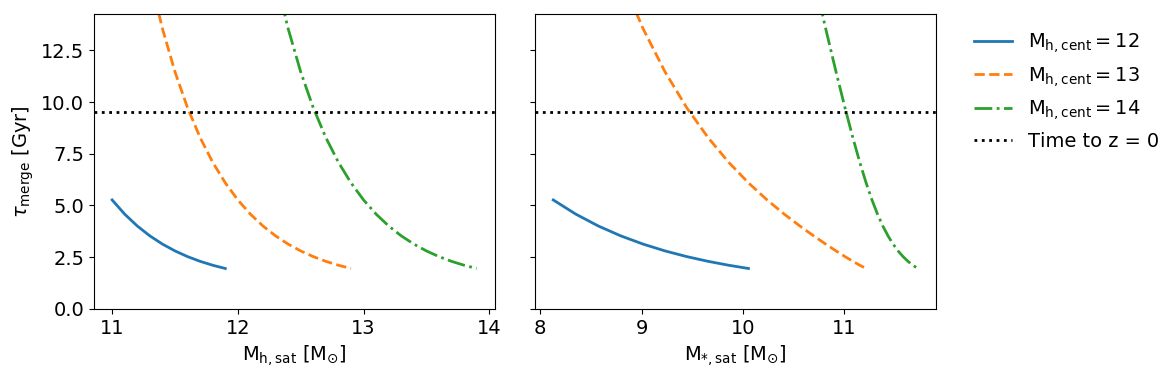
\includegraphics[width = \linewidth]{Figures/Chapter3/Tdyn_M.png}
    \caption{The range of merging timescales for a range of subhalo (left) and satellite (right) masses when accreted at $z = 1.5$ onto three different host masses: $\log$ $M_{h, cen}$ $[M_{\odot}]$ = 12 (blue solid), 13 (orange dashed) and 14 (green dot-dashed). The dotted black line shows the time to redshift $z = 0$, i.e. the minimum amount of time a satellite would need to survive to be observable in the local universe.}
    \label{fig:Tdyn_M}
\end{figure}

In Figure \ref{fig:AccretionTime} the practical effect of increasing the dynamical time is shown. Increasing the dynamical time factor $f_{tdyn}$ to infinity, satellites will never merge with the central and thus the left-hand panel shows the total buildup of satellites over cosmic time. In the right-hand panel, with $f_{tdyn} = 1$, we see how the population of satellites still observable at $z=0.1$ is built up over time. As expected from Figure \ref{fig:Tdyn_M}, only recently accreted massive satellite galaxies contribute to the observable population whereas smaller galaxies will have a wider distribution of accretion times. Notably, there are no galaxies, within our mass ranges, accreted before redshift $z=2$ that remain observable at redshift $z=0.1$.

\begin{figure}[h]
    \centering
    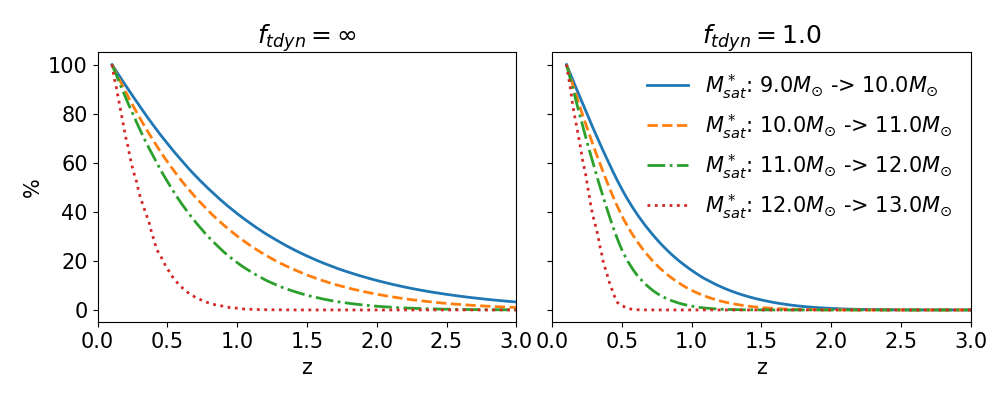
\includegraphics[width = \linewidth]{Figures/Chapter3/AccretedSatellitePercentage.png}
    \caption{We show the percentage of satellites observed at a $z = 0.1$ as a function of their redshift of accretion $z > 0$. It can be seen that massive satellites observed at $z = 0.1$ are accreted more recently than smaller satellites. At $z = 0.5$ less that 50\% of the total satellites observed at $z = 0.1$ have been accreted, and at $z = 0.1$ this falls to less than 20\%. }
    \label{fig:AccretionTime}
\end{figure}

\subsection{Effects of Dynamical Friction}
%Show the dynamical friction model and how that actually impacts the distribution.
In this Section, we show the prediction of \steel with different merging timescales, $f_{tdyn}$ = $0.5, 1.0, 2.5$, to probe the effects of dynamical time on the satellite population. In Figure \ref{fig:SMF_Tdyn} we find, as expected, that longer dynamical times tend to increase satellite number densities especially towards lower stellar masses. The number densities of higher-mass satellites are more resilient to increase with dynamical time. In fact, when $f_{tdyn}\gtrsim 1$ the number densities of massive satellites become already very close to the theoretical maximum number density when  $f_{t_{dyn}} = \infty$. This trend is also seen in Figure \ref{fig:AccretionTime}, the difference between the buildup of high mass satellites between $f_{t_{dyn}} = \infty$ and $f_{t_{dyn}} = 1$ is much less significant than between that of low mass satellites.
It follows that massive satellites are on average a recently accreted population. In other words, there are only a few high mass satellites that had enough time to merge when $f_{tdyn}\gtrsim 1$. In contrast, lower mass satellites have not yet reached their theoretical limit, and thus they can still increase their number densities with increasing dynamical time.  

When computing the distribution of satellites as a function of parent halo mass we show both full number densities, as well as fractional distributions to better highlight the ``skewness'' of the predicted distributions with respect to the data. The latter will be simply computed as
\begin{equation}
\label{eqn:FracPlot}
F(dM_h) = \frac{N(>10^x)|_{dM_h}}{N(x)},
\end{equation} 
where $N(>10^{x})$ is the total number (density) of satellites above a threshold stellar mass $x= \log M_{*}$, and the $N(>10^{x})|_{dM_h}$ is the number of these that reside within the halo mass bin $[M_h, M_h+dM_h]$.

Figure \ref{fig:Sat_Dist_Tdyn} shows how as a function of parent halo mass the distribution of satellites, above three stellar-mass cuts, is affected by $f_{tdyn}$. The number density distribution (top row) shows results similar to the satellite SMF where increasing dynamical time increases the number densities. However, there is also an apparent steepening effect for which lower mass host haloes end up containing relatively fewer satellites with respect to models with longer dynamical times. The fractional plot (bottom row) accentuates this change in the number density distributions shown in the top row: shorter dynamical times shift the peak of the distribution to the right as relatively more satellites are observed in high mass host haloes.

This steepening of the satellite distribution as a function of halo mass, as well as the shift of the peak in the lower row, where infinite dynamical times move satellites preferentially to lower halo masses, are both caused by the amount of time satellites survive in their hosts. Massive satellites are far more common in massive hosts, as can be inferred from the SHMF. Therefore, irrespective of the chosen merging timescale, there will always be a high number density of surviving massive satellites in higher mass parent haloes. However, when merging timescales are increased, the lower number densities of massive satellites in moderately-sized haloes are also increased. Given that lower mass parent haloes are more abundant, the reduction of merging timescales tends to shift the peak of the fractional distribution of galaxies to lower mass parents. Otherwise put, the merging timescales in clusters ($ \log_{10} M_{h,cent}$ $[M_{\odot}]$ $> 13.75$) are so long that even a factor five reduction in merger timescale still does not give the satellite galaxies sufficient time to merge with the central galaxy. This effect can be inferred from Figure \ref{fig:Tdyn_M}, where we see steeper gradients for a given subhalo/satellite mass with increasing parent halo mass. Merging is more efficient for the lower mass satellites as can be seen by the steepness of the $f_{t_{dyn}} = 0.5$ model (dashed lines) in the top row of Figure \ref{fig:Sat_Dist_Tdyn}.

%dynamical distributions

\begin{figure}[h]
    \centering
    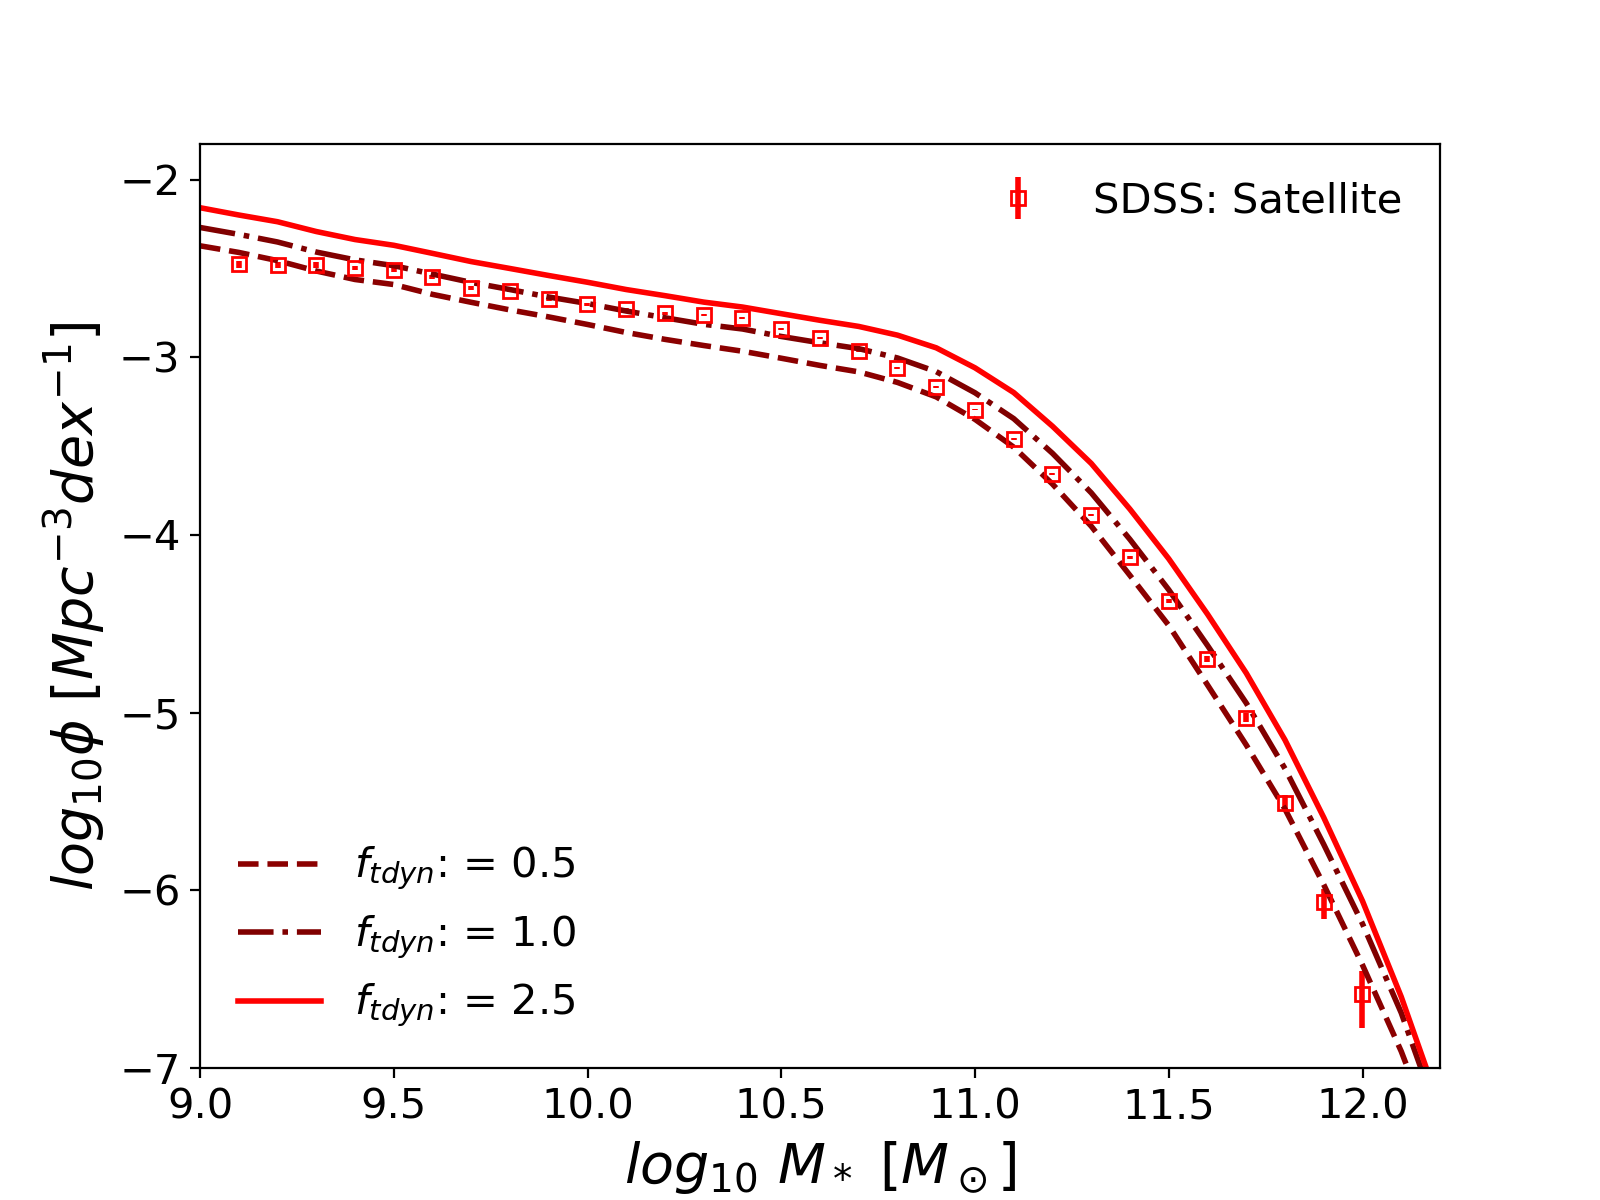
\includegraphics[width = \linewidth]{Figures/Chapter3/Tdyn_SMF.png}
    \caption{Satellite stellar mass functions generated by the model compared to SDSS data (open squares). The solid, dot dashed, and dashed lines show $f_{tdyn} = 0.5, 1.0,$ and $2.5$ respectively.}
    \label{fig:SMF_Tdyn}
\end{figure}

\begin{figure}[h]
    \centering
    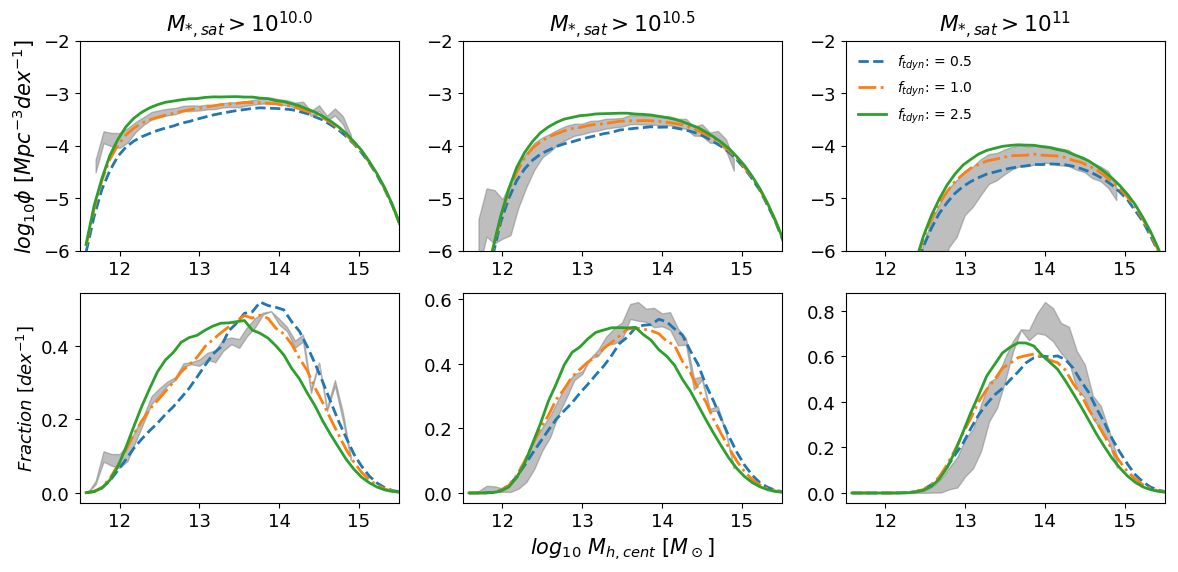
\includegraphics[width = \linewidth]{Figures/Chapter3/Tdyn_Sat_Dist.png}
    \caption{Satellite distributions in parent haloes generated from \steel are compared to those observed in SDSS (grey band). Columns from left to right show increasing satellite stellar mass cuts as labelled. The top row shows the number density of satellites expected to be found in each parent halo mass. The bottom row shows the fractional distribution described by Equation \ref{eqn:FracPlot}. The dashed, dot dashed, and solid lines show $f_{tdyn} = 0.5, 1.0,$ and $2.5$ respectively. The width of the grey band corresponds to a 10\% uncertainty in satellite stellar masses.}
    \label{fig:Sat_Dist_Tdyn}
\end{figure}

The least-square residuals to the SMF, number density distribution and fractional distributions are given in Table \ref{tab:bestfit}. There is no model that simultaneously fully matches all the observations in all mass ranges. The trend in both the number density distribution and the fractional distribution is that slightly longer dynamical times ($f_{tdyn}  = 1.2$) are favoured by the less massive satellites. Longer dynamical timescales better match the halo mass distributions (number density distribution/fractional distributions) for lower mass satellites, and vice versa for higher mass satellites with $\log M_{*}/M_{\odot} >11$. Nevertheless, the simple combination of abundance matching and dynamical merging timescales as suggested by pure N-body simulations ($f_{t_{dyn}} = 1.0$) tends to provide overall good agreement to both the satellite SMF and the satellite distributions, without the need to invoke additional physics in the (late) evolution of satellite galaxies after infall.

\begin{table*}
\centering
\caption{We show the sum of the squared residuals between the SDSS and our model. The satellite SMF is calculated between 9.1 and 12.0 $M_{*}$. The SDF fit is calculated between 12 and 14.9 $M_h$ for the \textgreater10 and\textgreater10.5 plots, and between 12.5 and 14.9 $M_h$ for \textgreater11. The Fractional plot fit is calculated between 11.6 and 14.9 $M_h$.}
\label{tab:bestfit}
\begin{tabular}{c|c|ccc|ccc}
$f_{t_{dyn}}$   & SSMF   (Fig \ref{fig:SMF_Tdyn})               & \multicolumn{3}{c}{SDF  } \vline & \multicolumn{3}{c}{Fractional Distribution } \\
   &   (Fig \ref{fig:SMF_Tdyn})               & \multicolumn{3}{c}{ (Top Row Fig \ref{fig:Sat_Dist_Tdyn}) } \vline & \multicolumn{3}{c}{ (Bottom Row Fig \ref{fig:Sat_Dist_Tdyn})} \\ \hline
            \multicolumn{1}{l}{} \vline & \multicolumn{1}{l}{} \vline & \multicolumn{1}{l}{\textgreater{}10} & \multicolumn{1}{l}{\textgreater{}10.5} & \multicolumn{1}{l}{\textgreater{}11} \vline & \multicolumn{1}{l}{\textgreater{}10} & \multicolumn{1}{l}{\textgreater{}10.5} & \multicolumn{1}{l}{\textgreater{}11} \\ \hline
0.5    & 0.022   & 0.19  & 0.55    & 0.073    & 0.0042 & 0.0047 & 0.0078  \\
0.8    & 0.025   & 0.13  & 0.51    & 0.089    & 0.0020 & 0.0017 & 0.0054  \\
1.0    & 0.034   & 0.12  & 0.56    & 0.10     & 0.0015 & 0.0011 & 0.0050  \\
1.2    & 0.043   & 0.12  & 0.53    & 0.11     & 0.0015 & 0.00094& 0.0046  \\
1.5    & 0.054   & 0.12  & 0.52    & 0.13     & 0.0017 & 0.0010 & 0.0045                              
\end{tabular}
\end{table*}

%show stripping/SF routines and their effects
\subsection{Evolutionary models}

The prior section makes an implicit assumption that satellites do not evolve after infall. In this Section, we apply several evolutionary effects to the satellites assuming they have the same properties as centrals at infall but then evolve due to in-situ processes and in response to their environment.


\subsubsection{Star Formation Rates}
We use the star formation rate (SFR) parameterization from \citet{Lee2015A1.3} with parameters\footnote{These parameters are derived by fitting data from ZFORGE in combination with far-IR imaging from \textit{Spitzer} and \textit{Herschel} in the range $0.5<z<4$. In this work we extrapolate their fits down to $z = 0$, as this is consistent with the SFR measured by  \cite{Salim2007UVUniverse} at lower redshifts.} from \citet{Tomczak2016THE4} where $s_0$ and $M_0$ have units $log(M_{\odot})$ and $M_{\odot}$ respectively,

\begin{equation}
\begin{split}
\label{eqn:SFR}
\log[\psi(z, M_*)] &= s_0(z) - \log \Big[ 1 + \Big(\frac{M_*}{M_0(z)}\Big)^{-\alpha(z)}\Big] \\
s_0(z) &= 0.195 + 1.157z - 0.143(z^2) \\
\log[M_0(z)] &= 9.244 + 0.753z - 0.090(z^2) \\
\alpha(z) &= 1.118.
\end{split}
\end{equation}

As discussed, continuity-equation approaches are more realistic and physically-based techniques to model galaxy growth, as, by design, they avoid the observed discrepancies between the time-integrated SFR and the independently measured stellar mass function at any given epoch. The novelty in our continuity model with respect to previous work is that we do not tune the resulting star formation rate on the total stellar mass function but rather only on the stellar mass function of \textit{central} galaxies \footnote{Which is in turn iteratively constrained by matching the local stellar mass function of SDSS centrals.}. We use as input for our continuity equation the central SMF generated by the SMHM relation and the central HMF from \cite{Tinker2010THETESTS}. When considering the mass growth we must consider the mass loss, else the SFR is massively under-predicted. We use an instantaneous loss fraction of $40\%$. We also neglect the mass gained from mergers. However, as mergers would decrease the SFR calculated, this method should be considered an upper limit to the real SFR. The fit to the resulting SFRs is given by

\begin{equation}
\begin{split}
\label{eqn:SFR_CE}
\log(\psi(z, M_*)) &= s_0(z) - \log \Big[ 1 + \Big(\frac{M_*}{M_0(z)}\Big)^{-\alpha(z)}\Big] \\
s_0(z) &= 0.6 + 1.22z - 0.2(z^2) \\
\log(M_0(z)) &= 10.3 + 0.753z - 0.15(z^2) \\
\alpha(z) &= 1.3 - 0.1z.
\end{split}
\end{equation}

In all cases, the SFR is included in our models with a log-normal scatter of 0.3 dex \citep{Leja2015ReconcilingFunction}.


We also include the ability to quench star formation in satellite galaxies after infall. It has been suggested that satellites undergo a ``delayed-then-rapid'' quenching \citep{Wetzel2013GalaxyUniverse}. The latter model envisions that satellites continue to form stars at the same rate as central galaxies of comparable stellar mass for a time $\tau_q$ after infall, and then quench rapidly over a timescale $\tau_{f}$. This quenching is proposed for satellites with stellar mass above $M_*\gtrsim 10^9 M_{\odot}$, with a minimum $\tau_q$ $\sim$ $1$ $Gyr$. For galaxies below $M_* \lesssim 10^{9} M_{\odot}$, we however adopt the more recent results by \citet{Fillingham2016UnderStripping}, who put forward a parent halo mass dependent cutoff,
\begin{equation}
\label{eqn:Cutoff}
log(M_{cutoff}) = 9 log(M_{\odot}) - (15 log(M_{\odot}) - log(M_{h,host}))/5log(M_{\odot}) ,
\end{equation}
below which satellite galaxies all share the same quenching time $\tau_q=2$ Gyr.
The rapid quenching timescale $\tau_{f}$ can be expressed as \citep{Wetzel2013GalaxyUniverse},
\begin{equation}
\label{eqn:tauf}
\tau_f = -0.5 log(M_{*,sat}) + 5.7 Gyr.
\end{equation}
We set a minimum $\tau_{f}$ of $0.2$ $Gyr$ for all galaxies. This rapid quenching begins at times $t > \tau_q$ after infall, and it is approximated by an exponential decay which is longer for larger satellites, as can be inferred from Equation \ref{eqn:SFR_Quench}. The look-back time at which a galaxy begins fast quenching is then $t_q = t_{infall} - \tau_q$. After this time the satellite no longer follows the SFR of a typical central galaxy. Figure \ref{fig:QuenchFig} illustrates the quenching model where the dashed/coloured lines mark the halo mass dependence in cutoff mass.

\begin{figure}
    \centering
    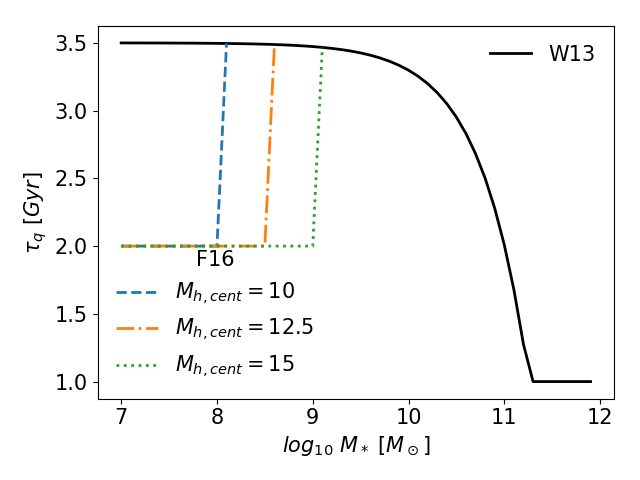
\includegraphics[width = \linewidth]{Figures/Chapter3/Fig4.png}
    \caption{The solid line shows the \citet[][W13]{Wetzel2013GalaxyUniverse} model for quenching. The dashed lines show the host halo dependent reduction in quenching time from \citet[][F16]{Fillingham2016UnderStripping} for three example host masses $\log10$ $M_{h, cent} = 10, 12.5, 15$ as labelled. Larger hosts are able to reduce the quenching time of larger satellites}.
    \label{fig:QuenchFig}
\end{figure}

The SFR during the satellite infall is then given by,

\begin{equation}
\label{eqn:SFR_Quench}
SFR(t, M_*) = SFR(t, M_*)
\begin{dcases}
\psi(z(t), M_*), & \text{} t > t_q \\
\psi(z(t_q), M_*)e^{\big[-\frac{t_q-t}{\tau_f}\big]}. & \text{} t < t_q
\end{dcases}
\end{equation}

If at any point a satellite galaxy has a SSFR below $10^{-12}$ $M_{\odot}$ $yr^{-1}$, it is assumed to be fully quenched and assigned a SSFR of $10^{-12}$ $M_{\odot}$ $yr^{-1}$, plus a log-normal scatter of 0.3 dex.


The first, purely observationally-based, star formation rate model strictly follows the SFR parametrization by \citet[][T16 hereafter]{Tomczak2016THE4}, given in Equation \ref{eqn:SFR}. The second star formation rate model (which we label as ``CE'') is instead based on the continuity equation approach. 

\begin{figure}
    \centering
    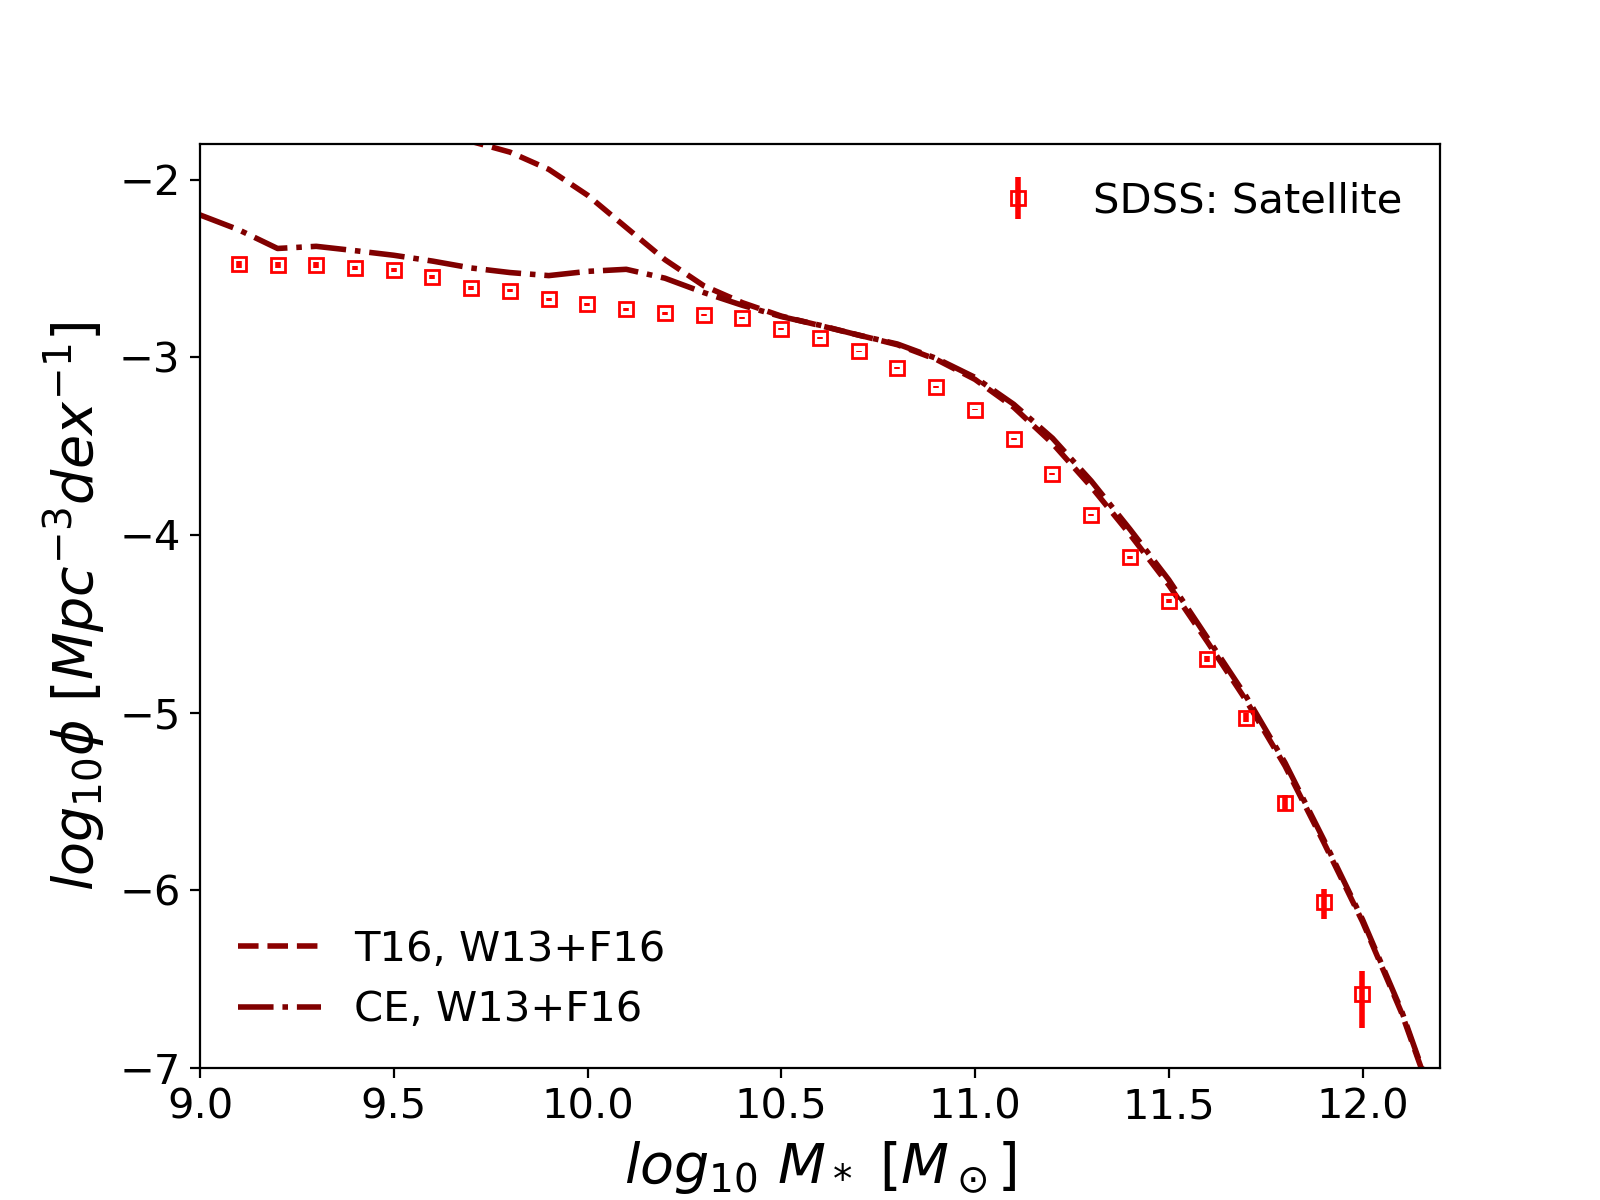
\includegraphics[width = \linewidth]{Figures/Chapter3/Fig9.png}
    \caption{Satellite stellar mass functions generated from the model using both the \citet{Tomczak2016THE4} (dashed) and continuity (dot dashed) star formation rates compared to the SDSS satellite stellar mass function (open squares).}
    \label{fig:SMF_SF_Q}
\end{figure}

We compare the satellite SMFs produced by the two star formation+quenching models addressed above to our SDSS stellar mass function of satellites in Figure \ref{fig:SMF_SF_Q}. It is apparent that using the observed SFR by T16 (dashed line), even inclusive of the best recipes for quenching, still substantially overproduces the number density of galaxies below $M_* \lesssim 3\times 10^{10}\, M_{\odot}$. This is a well-known problem affecting the full (dominated by central) galaxy population \citep[e.g.,][]{Leja2015ReconcilingFunction}: the integrated (observed) SFR is not consistent with the moderate growth over time of the SMF causing an overproduction of galaxies becoming gradually more severe at lower stellar masses. Our results show a similar problem affecting the satellite population, on the assumption that the latter at infall share the same SFR distribution as a typical central galaxy of the same stellar mass.


We now show the relative impact of the star formation rate and stellar stripping on the satellite stellar mass function. Figure \ref{fig:SMF_SF_Strip} and Figure \ref{fig:Sat_Dist_SF_Strip} show stellar mass function and host halo mass distributions for the $f_{tdyn} = 1.0$ reference model with no stripping nor star-formation, the CE star formation model, and the CE star formation model with stripping (long-dashed, dot-dashed, and solid lines, respectively). We see from both Figures that the reference and star-formation model are almost indistinguishable. The stripping, at least at the level implemented in this work, also has a rather minor effect, at the most reducing the number densities of the most massive satellites ($>10^{11}M_{\odot}$) by $\lesssim 0.2$ dex.

\begin{figure}
    \centering
    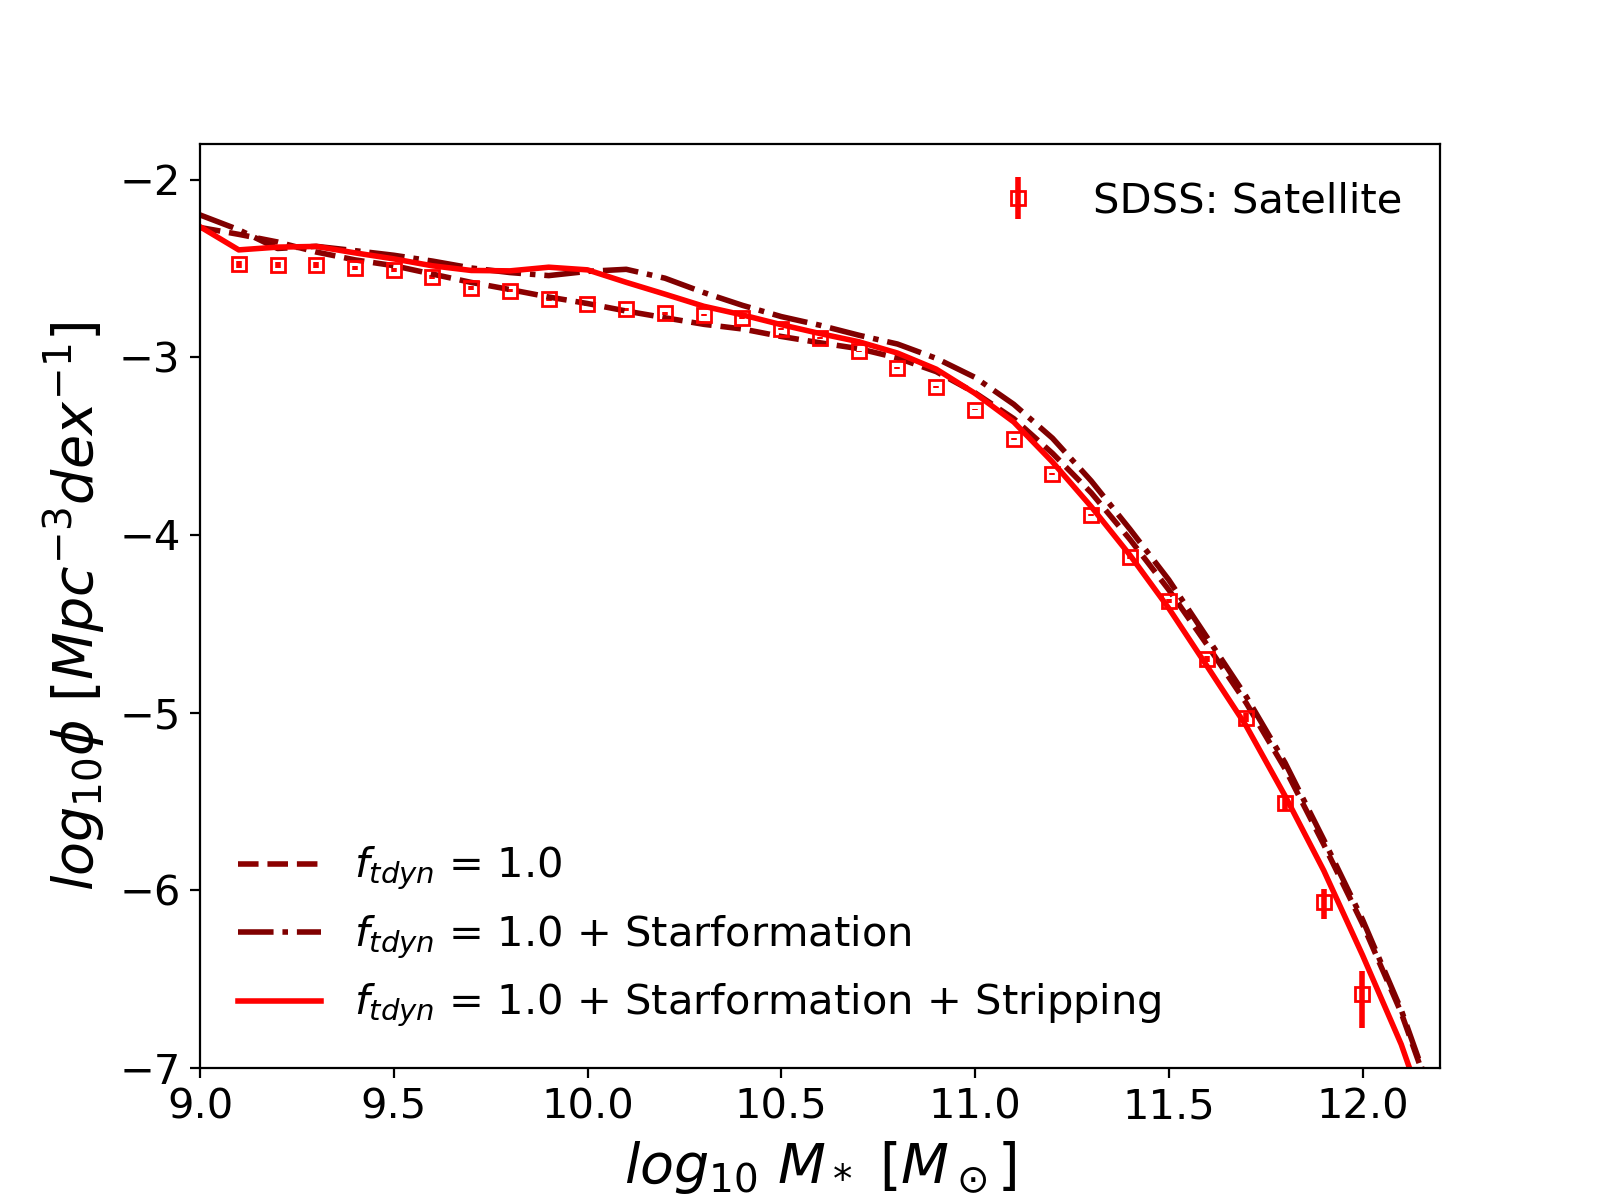
\includegraphics[width = \linewidth]{Figures/Chapter3/Fig11.png}
    \caption{Satellite stellar mass functions generated from the model compared to SDSS satellites (open squares). The models shown all have $f_{tdyn} = 1.0$ and are the reference `frozen model' (dashed line), starformation (CE model) only (dot dashed line) and starformation and stripping (solid line).}
    \label{fig:SMF_SF_Strip}
\end{figure}

\begin{figure}
    \centering
    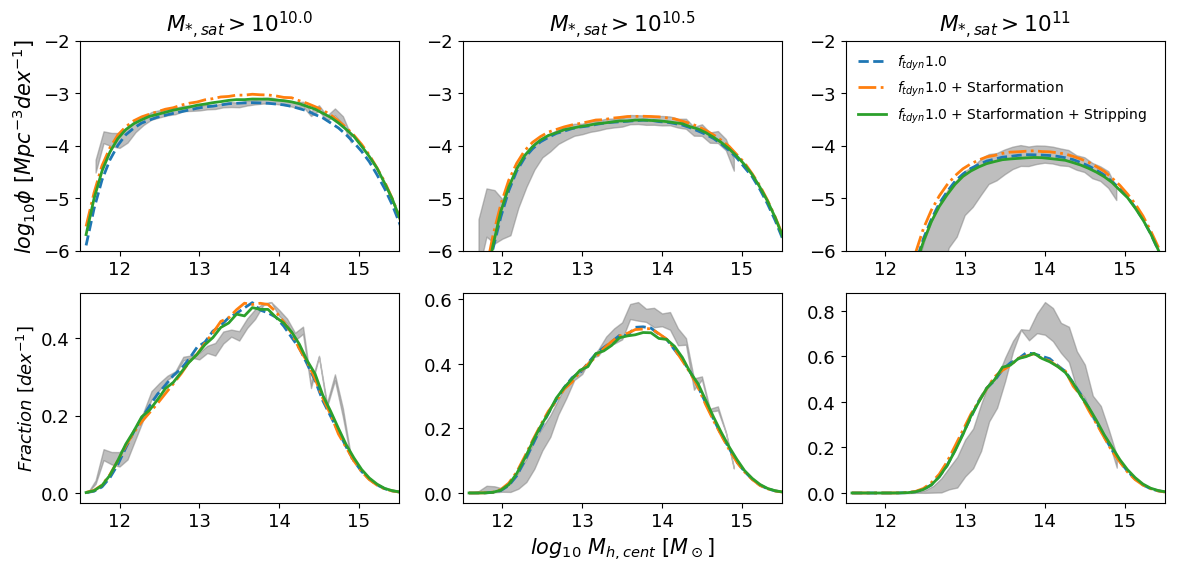
\includegraphics[width = \linewidth]{Figures/Chapter3/Sat_Dist_SF_Strip.png}
    \caption{Satellite distributions in parent haloes generated from the model are compared to those observed in SDSS (grey bands). Columns from left to right show increasing satellite stellar mass cuts as labelled. The top row shows the number density of satellites expected to be found in each parent halo mass. The bottom row shows the fractional distribution described by Equation \ref{eqn:FracPlot}. The models shown all have $f_{tdyn} = 1.0$ and are the reference 'frozen model' (dashed line), star formation only (dot dashed line) and star formation and stripping (solid line). The width of the grey band corresponds to a 10\% uncertainty in satellite stellar masses.}
    \label{fig:Sat_Dist_SF_Strip}
\end{figure}

\begin{table*}
\centering
\caption{We show the sum of the squared residuals between the SDSS and our model as in \ref{tab:bestfit} with the same mass ranges for the fitting. All models have $f_{t_{dyn}} = 1.0$ from top to bottom we then have the reference frozen model, the model with starformation, and the model with stripping and starformation.}
\label{tab:SF_Strip}
\begin{tabular}{c|c|ccc|ccc}
$f_{t_{dyn}}$   & SSMF   & \multicolumn{3}{c}{SDF  } \vline & \multicolumn{3}{c}{Fractional Distribution } \\
   &   (Fig \ref{fig:SMF_SF_Strip})               & \multicolumn{3}{c}{ (Top Row Fig \ref{fig:Sat_Dist_SF_Strip}) } \vline & \multicolumn{3}{c}{ (Bottom Row Fig \ref{fig:Sat_Dist_SF_Strip})} \\ \hline
            \multicolumn{1}{l}{} \vline & \multicolumn{1}{l}{} \vline & \multicolumn{1}{l}{\textgreater{}10} & \multicolumn{1}{l}{\textgreater{}10.5} & \multicolumn{1}{l}{\textgreater{}11} \vline & \multicolumn{1}{l}{\textgreater{}10} & \multicolumn{1}{l}{\textgreater{}10.5} & \multicolumn{1}{l}{\textgreater{}11} \\ \hline
1.0 & 
0.034 & 0.12 & 0.53 & 0.10 & 0.0015& 0.0011& 0.0049\\
\begin{tabular}[c]{@{}c@{}}1.0\\ With Star Formation\end{tabular} & 
0.049 & 0.077& 0.43 & 0.14 & 0.0018& 0.0012& 0.0059\\
\begin{tabular}[c]{@{}c@{}}1.0\\ With Stripping and Star Formation\end{tabular} & 
0.021 & 0.087& 0.47 & 0.088& 0.0016& 0.0015& 0.0056
\end{tabular}
\end{table*} 

Table \ref{tab:SF_Strip} shows the sum of the square residuals to the SMF, SDF and fractional distributions for the same models discussed above, our reference frozen one, and the one with evolution of satellites after infall (stellar stripping and continuity equation-based star formation). Table \ref{tab:SF_Strip} shows that the satellite late evolution has little effect on the fractional distribution. In the number density distribution we see an improved fit for galaxies in the $M_*>10^{11}\, M_{\odot}$ range, mainly induced by the stripping which slightly reduces the number density of massive galaxies. Table \ref{tab:SF_Strip} shows the sum of square residuals for the dynamical time with $f_{t_{dyn}}=1$, for the frozen and evolved models. 

\section{Multi-Epoch Distributions of Satellite Galaxies}

We here extend the group and cluster satellite richness analysis to high redshift. In Section \ref{sec:ObsSatDist} it is found that dynamical friction and, to a second-order, abundance matching, are the dominant factors in the distribution of satellite galaxies in groups and clusters above $M_{*,sat} > 10^{10} M_{\odot}$. Here we display the results for the full \textsc{steel} model which includes star formation, dynamical quenching and stripping to evolve satellites after infall. The latter effects, despite being of lower order than dynamical friction or abundance matching, are included to be able to compare to data other than cluster richness, such as the satellite specific star formation rate distribution.

\begin{figure}[h]
    \centering
    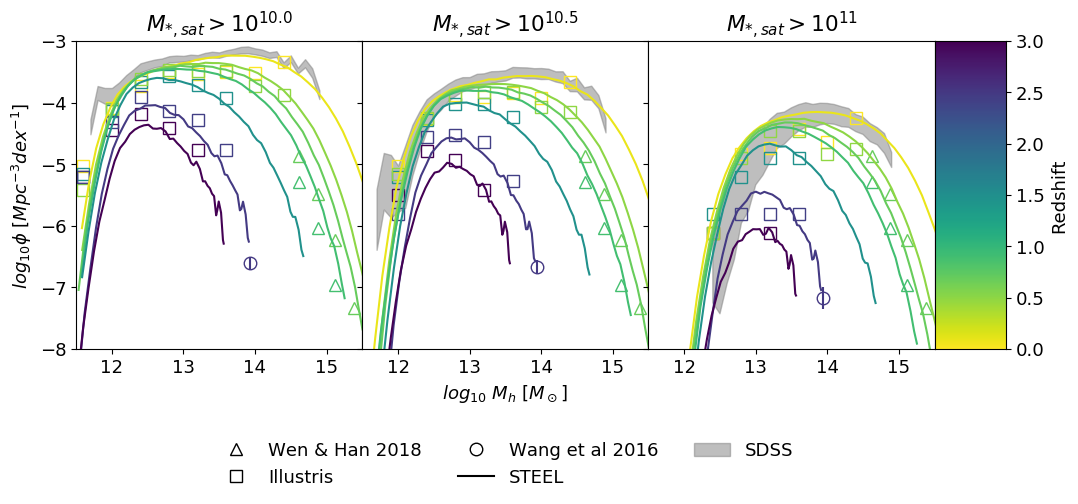
\includegraphics[width = \linewidth]{Figures/Chapter3/HighzClusters.png}
    \caption{The number-density distribution of satellites per parent halo mass predicted from \textsc{steel}, using the PyMorph SMHM relation, at multiple redshift epochs (solid lines). The grey band is the data from SDSS at redshift $z=0.1$. Also included are the high redshift cluster data from \citet{Wang2016DISCOVERY2.506} (circles) and \citet{Wen2018ARedshifts} (triangles). For completeness, the Figure also includes the outputs from the Illustris simulation using the TNG100 data (crosses). Each data point and line are given a colour associated to their redshift (the bar on the right provides the color coding key).}
    \label{fig:Sat_Dist_High_z}
\end{figure}

Figure \ref{fig:Sat_Dist_High_z} shows the satellite number density per halo mass bin. For each central halo mass the cosmic number density, similar to the number density presented in the cumulative stellar mass functions, is calculated for satellites above a mass threshold for each halo mass bin.
The predicted halo richness from \textsc{steel}, using the PyMorph SMHM relation, is shown in this plot as solid lines. The predictions from the Illustris TNG100 simulation \citep{Nelson2018FirstBimodality, Springel2018FirstClustering} are shown with crosses.  Low redshift SDSS data are shown as a grey band, cluster data detailed in Section \ref{subsec:Clusters} are open symbols. The markers and lines in the figure are colour coded based on redshift, as indicated by the colour bar on the right.

\section{Discussion}

There is a vast literature on the modelling of satellite galaxies. Here we recall examples of semi-empirical and semi-analytic models to highlight some of the key similarities and key differences. \citet{Neistein2013A2011}, with an approach similar to ours, separated the central and satellite populations in an attempt to better define the galaxy halo connection. By allowing in an N-body simulation the stellar mass of satellite galaxies to depend on both the host subhalo mass and the parent halo mass, \citet{Neistein2013A2011} find that the local satellite stellar mass-halo mass is substantially less well defined than the one for central galaxies. In our model satellites instead, strictly follow the stellar-mass-halo-mass relation of centrals at infall. In this way we find the resulting satellite distributions to be well reproduced. Our semi-empirical statistical model was able to reproduce multiple observables such as the stellar and parent halo mass distributions, with essentially only one parameter, $f_{t_{dyn}}$. By working with minimal assumptions and related free parameters, our approach is thus less prone to possible degeneracies affecting more traditional, multi-parameter techniques.

Another key difference with respect to previous models concerns ``orphan galaxies''. In N-body or merger tree-based simulations, when a subhalo drops below the resolution limit, an orphan galaxy is created \citep[e.g.,][]{Guo2011FromCosmology, DeLucia2011TimesCosmology}. It is then necessary to make an assumption on how much longer that subhalo (and hosted satellite galaxy) will survive. In our model, we avoid this complication by self-consistently assigning to all satellites a (full) observability timescale at infall.

We found in Figure \ref{fig:Sat_Dist_High_z} that \textsc{steel} is able to predict the existence of extreme objects. It is able to use rich cluster environments that are observable up to high redshift and contain some of the most massive galaxies as comparative data. This gives \steel an edge as exploring the richness of the environments around massive galaxies provides an excellent constraint to hierarchical assembly predicted by $\Lambda$CDM cosmology at the most extreme masses \citep{Shankar2015}. For example, we successfully compare with the cluster reported in \citet{Wang2016DISCOVERY2.506}, which other models \cite[e.g.][]{Henriques2015GalaxyMasses} have been unable to reproduce within a $\Lambda$CDM framework. However we concur with \citet{Wang2016DISCOVERY2.506} that these objects are rare (i.e. low number density) and their absence in traditional simulations could be simply attributed to poor statistics (i.e. small volumes) and not necessarily to the implied physical model. With large-scale surveys such as EUCLID coming online, a well-tuned statistical model could more easily place robust constraints on high-redshift cluster formation. 
 
In the following chapters we will use these tight constraints on the satellite distributions, and by extension satellite accretion rates, in conjunction with the statistical halo growth histories to test the total mass assembly statistics of galaxy populations. This is a departure from classical models which collect the assembly statistics for individual galaxies then take a population average. 
Additionally, we are able to use the flexible nature of a semi-empirical model to begin to look at how the SMHM relation can be used to understand systematic differences introduced by assumptions behind data analysis algorithms (such as M/L, IMF, etc...). The methodology presented in Chapter \ref{Chapter:Method} and the results in this chapter open the gates to novel analysis providing a unique view of the assembly of galaxies.
 
\subsection{Future work}
The quality of data presented in Figure \ref{fig:Sat_Dist_High_z}, SDSS and targeted cluster observations is a limitation to our ability to constrain the environments of galaxies over many epochs. The data limits the technique due to the lack of halo mass estimations and satellite/central identification in the high redshift data sets. To obtain the required data products accurate clustering analysis similar to that of \citet{Yang2012EvolutionHalos} must be applied to comprehensive high redshift surveys such as EUCLID. 

When comprehensive high redshift data sets with satellite/central identification are available, \steel will be well-positioned to place constraints on several aspects of hierarchical galaxy formation. Firstly, with good central SMF, the quality of abundance matching will improve significantly with the uncertainties regarding the contributions from satellite galaxies removed (Section \ref{C2:SubSec:AbnMtch}). The analysis of the impact of dynamical friction timescales on the exact shape of the satellite distributions such as that shown in Figure \ref{fig:Sat_Dist_Tdyn} can be extended to high redshift. Constraints on the dynamical friction timescales will improve estimations of the central galaxy accretion and merger rates that are further discussed in Chapters \ref{Chapter:GalGrowth} \& \ref{Chapter:GalPairs}.